\documentclass{egee}
%\usepackage{doxygen}

\usepackage{xspace}
%\usepackage{doxygen}

\def\LB{L\&B\xspace}
\def\JP{JP\xspace}
%\def\eg{e.\,g.}
\def\eg{for example\xspace}
\def\Eg{For example\xspace}
%\def\ie{i.\,e.}
\def\ie{that is\xspace}
\def\wrt{with respect to\xspace}
\def\Dash{---\penalty-1000}

\long\def\TODO#1{\par\noindent\textbf{TODO:} {\sl#1}\par}
\long\def\ludek#1{}

\hyphenation{plug-in}


\title{Job Provenance}
\Subtitle{Administrator's Guide}
\author{CESNET EGEE II JRA1 team}
\DocIdentifier{EGEE-II....}
\Date{\today}
\Activity{JRA1: Middleware Engineering and Integration}
\DocStatus{DRAFT}
\Dissemination{PUBLIC}
\DocumentLink{http://...}

\Abstract{ This administrator's guide explains how to administer the Job
Provenance (\JP) service. Several deployment scenarios are described together
with the installation, configuration, running and troubleshooting steps. }

\begin{document}

\begin{center}
{\bf Delivery Slip}
\end{center}
\begin{tabularx}{\textwidth}{|l|l|l|X|X|}
\hline
           & {\bf Name} & {\bf Partner} & {\bf Date} & {\bf Signature} \\
\hline
{\bf From} &                  &  & & \\
\hline
{\bf Reviewed by} & &  & & \\

\hline
{\bf Approved by} & & & & \\
\hline
\end{tabularx}

\begin{center}
{\bf Document Change Log}
\end{center}

\begin{tabularx}{\textwidth}{|l|l|X|X|}
\hline
{\bf Issue } & {\bf Date  } & {\bf Comment } & {\bf Author  } \\   \hline

\hline
\end{tabularx}

\begin{center}
{\bf Document Change Record}
\end{center}

\begin{tabularx}{\textwidth}{|l|l|X|}
\hline
{\bf Issue } & {\bf Item  } & {\bf Reason for Change } \\   \hline

\hline
\end{tabularx}

%
% Official text received on October 6, 2004
%
\vfill{\bf Copyright }\copyright{\bf Members of the EGEE Collaboration. 2004. 
See http://eu-egee.org/partners for details on the copyright holders. 

EGEE (``Enabling Grids for E-science in Europe'') is a project funded by
the European Union.  For more information on the project, its partners
and contributors please see http://www.eu-egee.org.

You are permitted to copy and distribute verbatim copies of this
document containing this copyright notice, but modifying this document
is not allowed. You are permitted to copy this document in whole or in
part into other documents if you attach the following reference to the
copied elements: ``Copyright }\copyright{\bf 2004. Members of the EGEE
Collaboration. http://www.eu-egee.org''

The information contained in this document represents the views of
EGEE as of the date they are published. EGEE does not guarantee that
any information contained herein is error-free, or up to date.

EGEE MAKES NO WARRANTIES, EXPRESS, IMPLIED, OR STATUTORY, BY
PUBLISHING THIS DOCUMENT.}


\clearpage

\newpage
\tableofcontents

\newpage
\section{Introduction}
\TODO{Do a reasonable merge with the JPUG-Introduction, do not duplicate text...}


\subsection{Job Provenance service overview}
The information about jobs submitted to gLite Workload Management
System is collected by the Logging and Bookkeeping (LB) service.
LB tracks jobs in terms of events and processes them in
a~real time to give overall view on the actual job state. The user may
query the bookkeeping server to obtain either the raw events or the
computed job state, she may also register for receiving notifications
on particular job state changes.

While the LB is intended to keep track of jobs during its lifetime, it
is not supposed to be used for long term archival of such data. The
Job Provenance (JP) service is designed to provide long-term storage
of all data related to job life and allow the end user to perform
data-mining in this data.
The JP is supposed to provide the permanent storage of
the job related information as stored within the \LB, to couple it with
the input sandboxes and other system oriented information necessary to
reproduce the environment where a~particular job run.

\subsubsection{Gathering data into Job Provenance}
Fig.~\ref{fig:psinter} depicts basic gLite middleware components and
their interaction with the Job Provenance.

\begin{figure}[htpb]
  \centering
  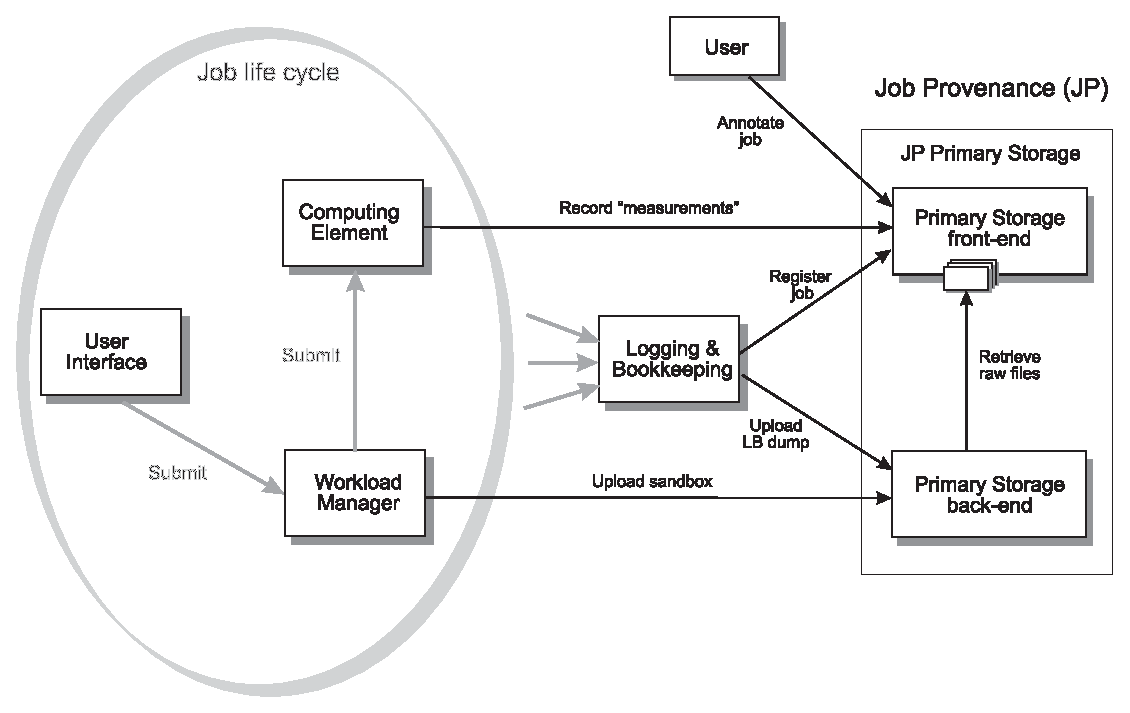
\includegraphics[scale=0.7]{JP-interactions}
  \caption{Data flow into gLite Job Provenance}
  \label{fig:psinter}
\end{figure}

JP is formed of two classes of services: permanent \emph{Primary
Storage} (JPPS) accepts and stores job data while possibly volatile
and configurable \emph{Index Servers} (JPIS) provide an optimized
querying and data-mining interface to the end-users.  The only direct
data retrieval scenario supported by JPPS is the case when user know exact ID
of jobs in the interest.

\subsubsection{Getting data from Job Provenance}

The role of \emph{Index Servers} (JPIS) is processing and re-arranging the data
from Primary Storage(s) into a~form suitable for frequent and complex user
queries. A user query part of JP is shown in Fig.~\ref{fig:query}.

\begin{figure}[htpb]
  \centering
  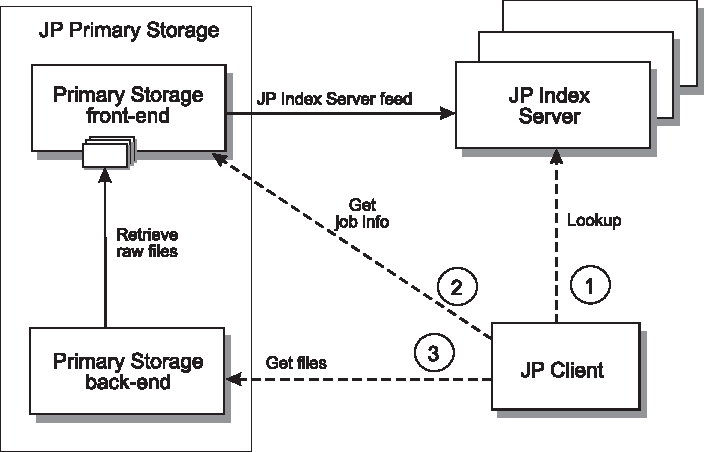
\includegraphics[scale=0.8]{JP-query}
  \caption{Index Server interactions}
  \label{fig:query}
\end{figure}

Index Servers are created, configured, and populated semi-dynamically
according to particular user community needs.  It is responsibility of
its administrator to setup the JPIS with appropriate configuration. There
is no prescribed relationship between Primary Storage and Index Server
installations.  An Index Server may retrieve data from multiple
Primary Storages and vice versa.

% TODO: update 
% The interface exposed by JPIS to the end user is described in the
% chapter~\ref{reference}. Command line interface tool for end-user
% interface to the JPIS is described in the chapter~\ref{CLI}.  See the
% next chapter (use cases) for futher description of JP to user
% interactions.


% LB-JP-interaction
\subsection{Interaction with Logging and Bookeeping (\LB)}

In this section we describe the interaction of JP with Logging and Bookkeeping
(\LB) service.  The data flows between LB and JP services are displayed in
Figure~\ref{fig:LB-JP-interactions}.  These flows are numbered and one can use
this numbers to find additional information about each flow in
table~\ref{tab:LB-JP-interactions}.

\begin{figure}[htpb]
  \centering
  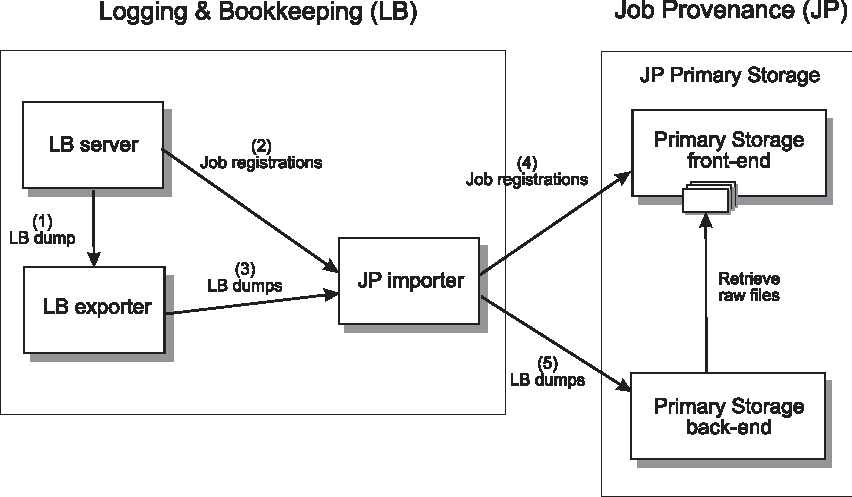
\includegraphics[width=0.9\hsize]{LB-JP-interaction-details}
  \caption{LB to JP interactions detail overview}
  \label{fig:LB-JP-interactions}
\end{figure}

\begin{table}[htpb]
 \centering
  \begin{tabular}{|c|p{3cm}|l|p{9cm}|}
    \hline
    &spool directory&initiated by&description\\
    \hline
    \hline
    1&lb.export.dump,
      lb.export.dump.keep&lb-exporter&
      Export of LB job records into spool directory. It uses glite-lb-purge utility. LB-exporter reads this spool directory in a regular manner and implement next processing of LB dumps. Optionally it can keep handled dumps in lb.export.dump.keep.\\
    \hline
    2&lb.export.jpreg&LB server&When new job come to the LB server 
    it stores its
    registration into the spool directory. It is responsibility of
    JP-importer process to handle such registrations.\\
    \hline
    3&lb.export.jpdump,
      lb.export.jobs,
      lb.export.jobs.keep&lb-exporter&
      LB-exporter do its processing of LB dumps (they are in per job form) and passes on it to the JP-importer using the spool directory lb.export.jpdump and temporary storage lb.export.jobs. It can keep the job files for futher usage.\\
    \hline
    4&none&jp-importer&JP importer handles registrations received from LB
    server and sends it to the JP primary server front-end (using its WS
    interface).\\
    \hline
    5&none&jp-importer&JP importer handles LB dumps received from LB
    exporter and sends it to the JP primary server back-end using its
    gridftp interface.\\
    \hline
  \end{tabular}
  \caption{LB to JP data flows description}
  \label{tab:LB-JP-interactions}
\end{table}


Notes:
\begin{itemize}
 \item Only JP Primary Storage (JPPS) server is involved in described
   data flows. JP Index Servers are not part of this picture (they are
   feeded via corresponding JPPS).
 \item Only flows number 4 and 5 are designed to be inter-host. All
   the other interactions assume the components are on the same host and
   do use access to a shared filesystem.
 \item Data flow number 1 use glite-lb-purge utility (see its
   documentation) and passes to it argument from lb.export.purgeargs
   clause of the deployment configuration file. This argument contain
   the timeouts controlling after how long period of time a job
   staying in a terminal state is to be purged from the LB server.
 \item The LB exporter have a feature to store LB job event dumps in a
   directory for further handling (e.g. for job statistic tool). This behaviour
   is controled by lb.export.jobs.keep deployment config file clause (leave
   this clause empty if you don't use dumps for futher handling).
 \item The LB exporter also have a feature to keep all handled LB
   dumps (in glite-lb-purge format) in filesystem. This feature is
   controlled by lb.export.dump.keep.
 \item LB exporter is not a deamon, it's periodic invocation is
   provided by cron deamon.
\end{itemize}



%
\subsection{Deployment scenarios}



\newpage
\section{Installation}
\TODO{}

\subsection{Complete RPMs description}
\subsection{Daemons description}
\subsection{CLI tools description}



\newpage
\section{Configuration}
\TODO{}

\subsection{JPPS}
\subsubsection{Setting up the MySQL database}


\subsection{JPIS}

\begin{alltt}
The JP-IS server daemon assume prior creation of its database. Simple tool
  for database creation is org.glite.jp.index/config/dbsetup.sh

customize startup script /etc/init.d/glite-jp-indexd (see below)
  and set up service startup using this script


Currently, configuration is done by command line options,  and
some hard-coded options.


The index server takes the following options:

./glite-jp-indexd [option]
        -d, --debug      don't run as daemon, additional diagnostics
        -q, --query-type hist/cont/both (default history)
        -n, --noauth     don't check user identity with result owner
        -m, --mysql      database connect string
        -p, --port       port to listen
        -i, --pidfile    file to store master pid
        -o, --logfile    file to store logs
        -x, --config     file with server configuration

The config file parameter is required. There is the example configuration in
$GLITE_LOCATION/etc/glite-jpis-config.xml.
\end{alltt}


\newpage
\section{Running and stopping the services}
\TODO{}

\subsection{Tests if everything works properly}



\newpage
\section{Troubleshooting}
\TODO{}

\subsection{Debugging}
\subsection{Fine tuning the performance}



\nocite{jgc}
\bibliographystyle{unsrt}
\bibliography{lbjp}

\end{document}
